\documentclass{article}

\usepackage{graphicx}
\usepackage{tikz}
\usepackage{tikzsymbols}
\usetikzlibrary{calc,patterns,shapes.geometric}
\pagestyle{empty}
\usepackage[margin=0pt]{geometry}
\geometry{papersize={14in,12in}}

\def\centerarc[#1](#2)(#3:#4:#5){\draw[#1] ($(#2)+({#5*cos(#3)},{#5*sin(#3)})$) arc (#3:#4:#5);}

\begin{document}
	\begin{figure}
		\centering
		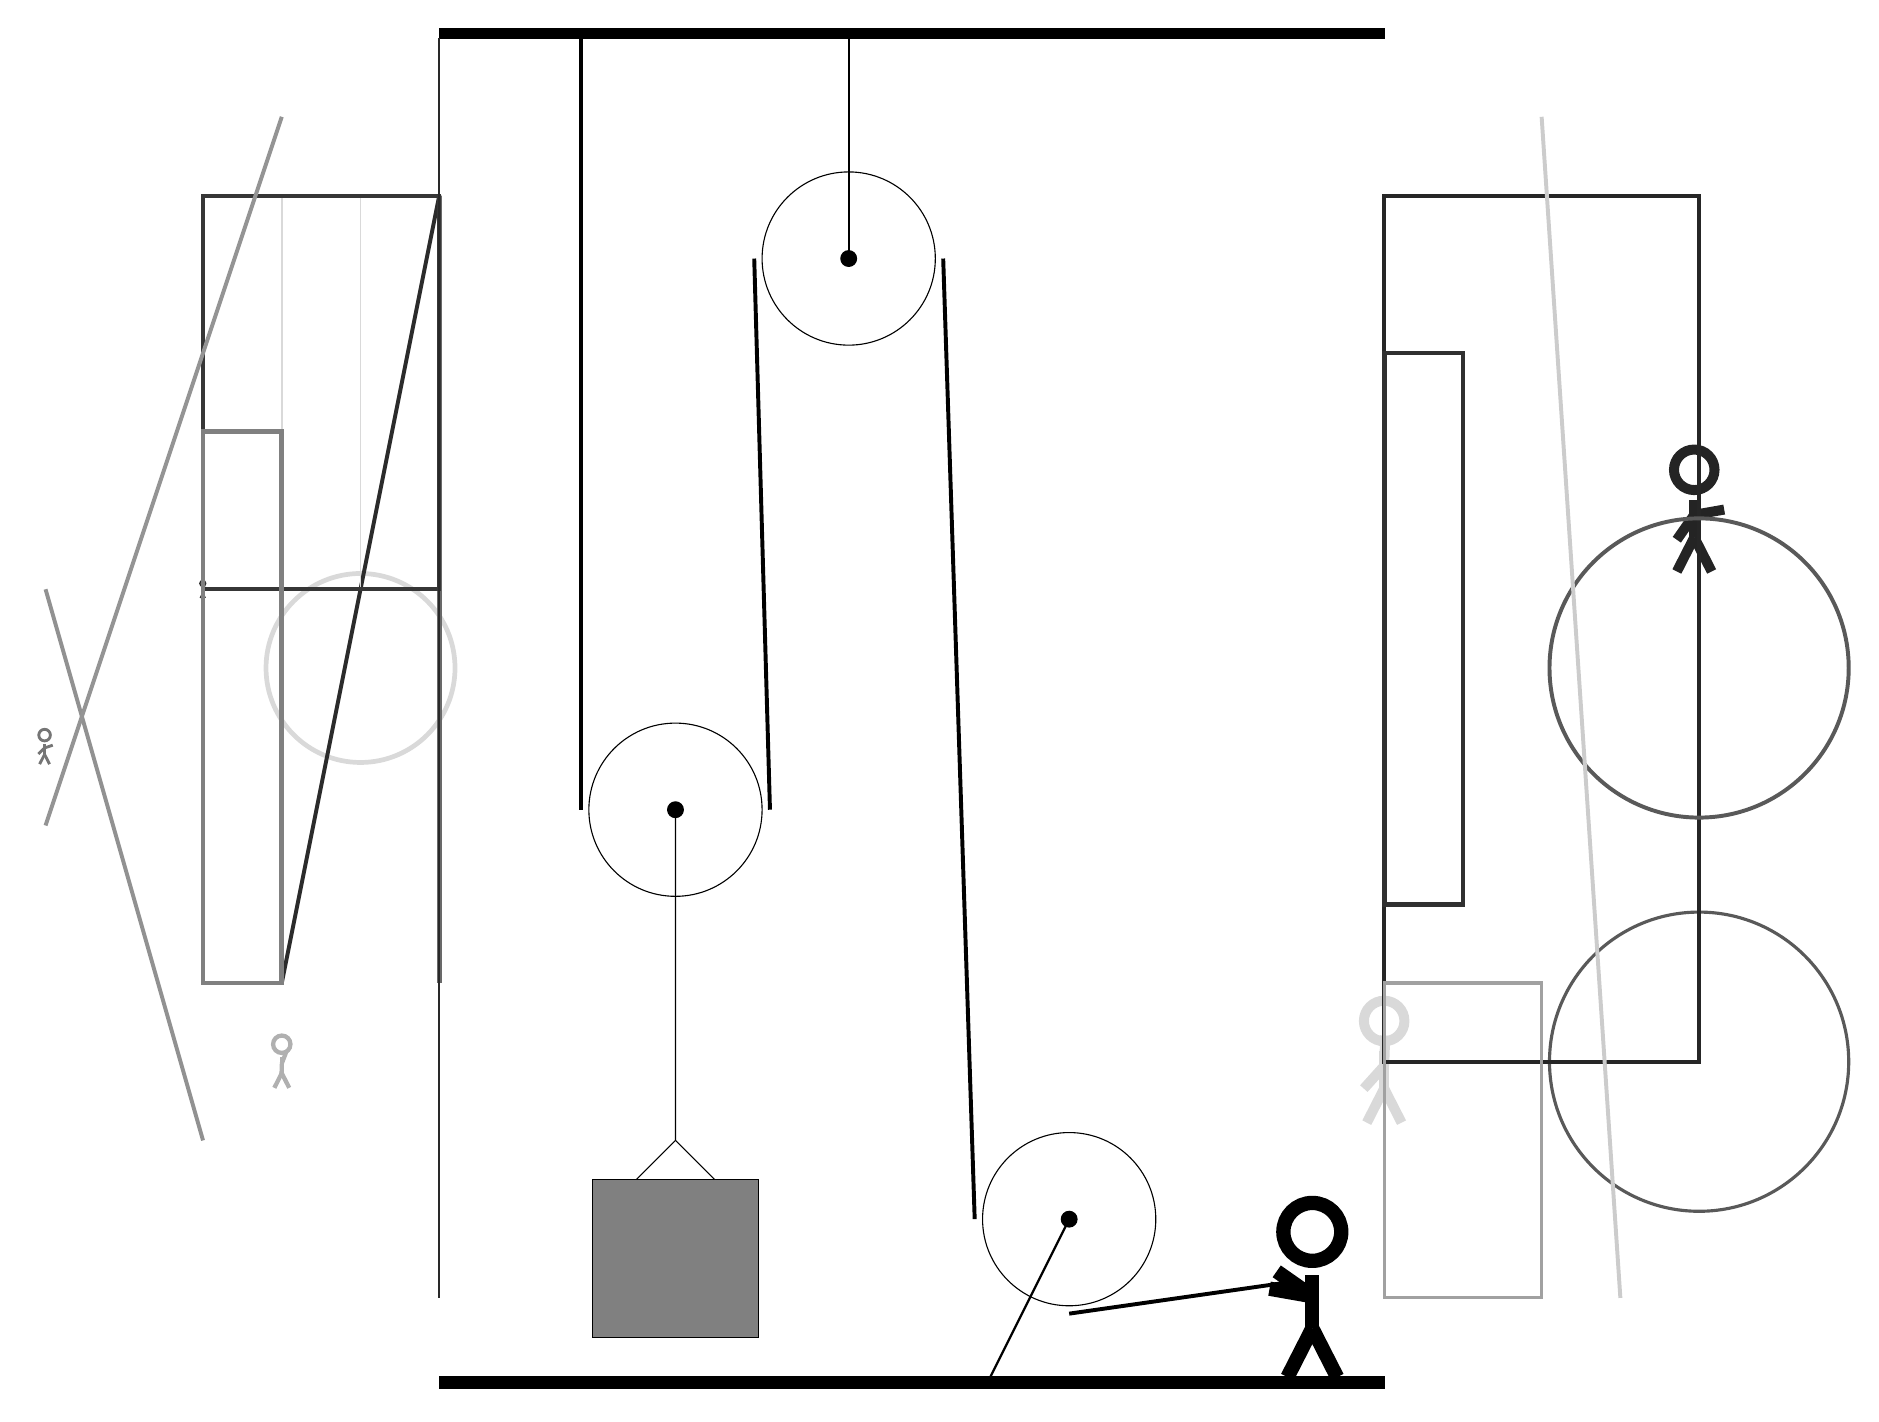
\begin{tikzpicture}
			%%%%% START %%%%%
			
			\draw[fill=black] (-2, 14) rectangle (10, 14.125);
			
			\draw (3.2, 11.2) circle (1.1);
			\draw[fill=black] (3.2, 11.2) circle (0.1);
			\draw[thick] (3.2, 11.2) -- (3.2, 14);
			
			\draw (6, -1) circle (1.1);
			\draw[fill=black] (6, -1) circle (0.1);
			\draw[thick] (6, -1) -- (5, -3);
			
			\node[line width=0.3mm, color=black!15] at (10, 1) {\Strichmaxerl[7][48][88]};
			
			\node[line width=0.5mm, color=black!31] at (-4, 1) {\Strichmaxerl[3][89][69]};
			\draw [line width=0.6mm, color=black!15](-3, 6) circle (1.2);
			\draw[line width=0.5mm, color=black!83](-2, 12) -- (-4, 2);
			\draw[line width=0.2mm, color=black!15] (-3, 7) rectangle (-4, 12);
			\draw[line width=0.5mm, color=black!43](-7, 7) -- (-5, 0);
			\draw[line width=0.7mm, color=black!59] (-2, 12) rectangle (-2, 2);
			\node[line width=0.2mm, color=black!86] at (14, 8) {\Strichmaxerl[7][55][10]};
			\draw [line width=0.4mm, color=black!65](14, 1) circle (1.9);
			\draw[line width=0.4mm, color=black!52] (10, 6) rectangle (10, 2);
			\draw[line width=0.5mm, color=black!79] (-2, 12) rectangle (-5, 7);
			
			\draw[line width=0.5mm, color=black!85] (10, 1) rectangle (14, 12);
			\node[line width=0.3mm, color=black!81] at (-5, 7) {\Strichmaxerl[1][78][38]};
			
			\draw[line width=0.5mm, color=black!42](-7, 4) -- (-4, 13);
			\draw[line width=0.6mm, color=black!50] (-4, 2) rectangle (-5, 9);
			\draw [line width=0.5mm, color=black!65](14, 6) circle (1.9);
			
			\draw[line width=0.3mm, color=black!84] (-2, -2) rectangle (-2, 14);
			\node[line width=0.3mm, color=black!54] at (-7, 5) {\Strichmaxerl[2][44][19]};
			\draw[line width=0.4mm, color=black!37] (12, -2) rectangle (10, 2);
			\draw[line width=0.6mm, color=black!81] (11, 10) rectangle (10, 3);
			\draw[line width=0.5mm, color=black!20](13, -2) -- (12, 13);
			
			\draw [line width=0.7mm, color=black!36](14, 6) circle (0.0);
			
			
			\draw (1, 4.2) circle (1.1);
			\draw[fill=black] (1, 4.2) circle (0.1);
			
			\draw (1, 4.2) -- (1, 0) -- (0.5, -0.5);
			\draw (1, 0) -- (1.5, -0.5);
			\draw[fill=black!50] (-0.05, -0.5) rectangle (2.05, -2.5);
			
			\draw[line width=0.5mm] (-0.2, 14) -- (-0.2, 4.2);
			\centerarc[line width=0.5mm](1, 4.2)(180:360:1.2000000000000002);
			\draw[line width=0.5mm](2.2, 4.2) -- (2.0, 11.2);
			\centerarc[line width=0.5mm](3.2, 11.2)(0:180:1.2000000000000002);
			\draw[line width=0.5mm](4.4, 11.2) -- (4.8, -1);
			\centerarc[line width=0.5mm](6, -1)(180:270:1.2000000000000002);
			\draw[line width=0.5mm](6, -2.2) -- (8.8, -1.8);
			
			\node at (9, -1.9) {\Strichmaxerl[10][-35][170]};
			
			\draw[fill=black] (-2, -3) rectangle (10, -3.15);
			
			%%%%% END %%%%%
		\end{tikzpicture}
	\end{figure}	
\end{document}